\chapter{Notions d'algèbre linéaire}

L'algèbre linéaire, c'est à la base une collection d'outils mathématique pour traiter plusieurs fonctions/opérations en parallèle. 

\begin{figure}[htbp]
	\centering
		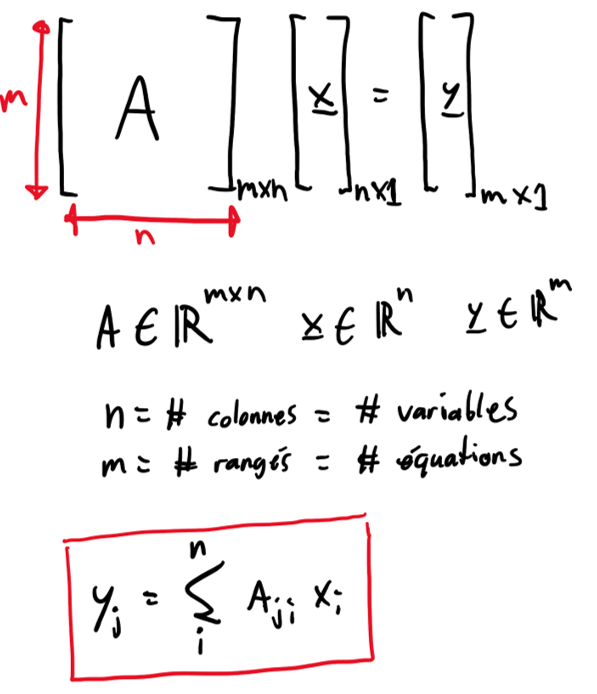
\includegraphics[width=0.70\textwidth]{calculmatriciel.png}
	\caption{Calcul matriciel }
	\label{fig:calculmatriciel}
\end{figure}


%%%%%%%%%%%%%%%%%%%%%%%%%%%%%%%%%%%%%%%%%%%%%%%%%%%%%
\newpage
\section{Système d’équations}
\label{sec:syseq}
%%%%%%%%%%%%%%%%%%%%%%%%%%%%%%%%%%%%%%%%%%%%%%%%%%%%%

Les opérations matricielles permettent de traiter plusieurs fonctions (linéaires) en parallèle. Par exemple, deux fonctions linéaires, $f_1$ et $f_2$, de deux variables (entrées), $x_1$ et $x_2$, peuvent s’écrire :
%
\begin{align}
y_1 = f_1(x_1,x_2) = a_{11} \, x_1 + a_{12} \, x_2   \\
y_2 = f_2(x_1,x_2) = a_{21} \, x_1 + a_{22} \, x_2
\end{align}
%
ou $y_1$ et $y_2$ sont les variables résultats (sorties) des fonctions, et $a_{ii}$ les paramètres internes des fonctions. Ces équations, avec la notation matricielle prennent la forme:
%
\begin{align}
\left[ \begin{array}{c} 
	y_1 \\ y_2
\end{array} \right] &= 
\left[ \begin{array}{c c} 
a_{11} & a_{12} \\ a_{21} & a_{22}
\end{array} \right]
\left[ \begin{array}{c} 
	x_1 \\ x_2
\end{array} \right] \quad \leftrightarrow \quad  \col{y}  =   A  \col{x} 
\label{eq:sys2}
\end{align}
%
ou $\col{y}$ et $\col{x}$ sont des vecteur-colonnes de dimension 2 et $A$ est une matrice 2x2. De façon générale, une matrice d'un tel système d’équation a une largeur $n$, correspondant au nombre de variable dans les équations, et une hauteur $m$, correspondant au nombre d’équations.
%
\begin{align}
\left[ \begin{array}{c} 
	y_1 \\ \vdots \\ y_m
\end{array} \right] &= 
\left[ \begin{array}{c c c} 
a_{11} & ... & a_{1n} \\ \vdots & \ddots  &  \vdots \\ 
a_{m1} & ... & a_{mn}
\end{array} \right]
\left[ \begin{array}{c} 
	x_1 \\ \vdots \\ x_n
\end{array} \right] \\
m: \quad \text{nombre de ranges} \quad&=\quad \text{nombre d’équations / sorties} \\
n: \quad \text{nombre de colonnes} \quad&=\quad \text{nombre de variables / entrées}
\end{align}
%


%%%%%%%%%%%%%%%%%%%%%%%%%%%%%%%%%%%%%%%%%%%%%%%%%%%%%
\section{Combinaison de vecteur-colonnes}
\label{sec:combveccol}
%%%%%%%%%%%%%%%%%%%%%%%%%%%%%%%%%%%%%%%%%%%%%%%%%%%%%

La multiplication d'une matrice par un vecteur-colonne peut être vue comme une combinaison linéaire des vecteur-colonnes de la matrice. Cette interprétation est très importante pour comprendre toutes les propriétés importantes et utiles des matrices, qui seront détaillées dans les prochaines sections. L’équation \eqref{eq:sys2}, correspondant a la multiplication d'un vecteur-colonne de dimension 2 par une matrice $2\times2$ peut être réécrite comme l'addition pondérée des deux colonnes de la matrice:
%
\begin{align}
\left[ \begin{array}{c} 
	y_1 \\ y_2
\end{array} \right] &= 
\left[ \begin{array}{c c} 
a_{11} & a_{12} \\ a_{21} & a_{22}
\end{array} \right]
\left[ \begin{array}{c} 
	x_1 \\ x_2
\end{array} \right] \quad \leftrightarrow \quad  \col{y}  =   
%
\underbrace{\left[ \begin{array}{c} 
	a_{11} \\ a_{21}
\end{array} \right]}_{\col{c}_1} \, x_1 +
\underbrace{\left[ \begin{array}{c} 
	a_{12} \\ a_{22}
\end{array} \right]}_{\col{c}_2} \, x_2
\label{eq:sys2-col}
\end{align}
%
Graphiquement, tel illustré à la figure \ref{fig:lincomb}, la multiplication d'une matrice peux être représenté par une addition pondérée (combinaison linéaire) des vecteurs correspondants aux colonnes de la matrice, dans l'espace sortie $\col{y} \in \re^m$.

%%%%%%%%%%%%%%%%%%%%%%%%%%%%%%%%%%%%%%%%%%%%%%%%%%%%%%%%%%%%
\begin{figure}[H]
	\centering
		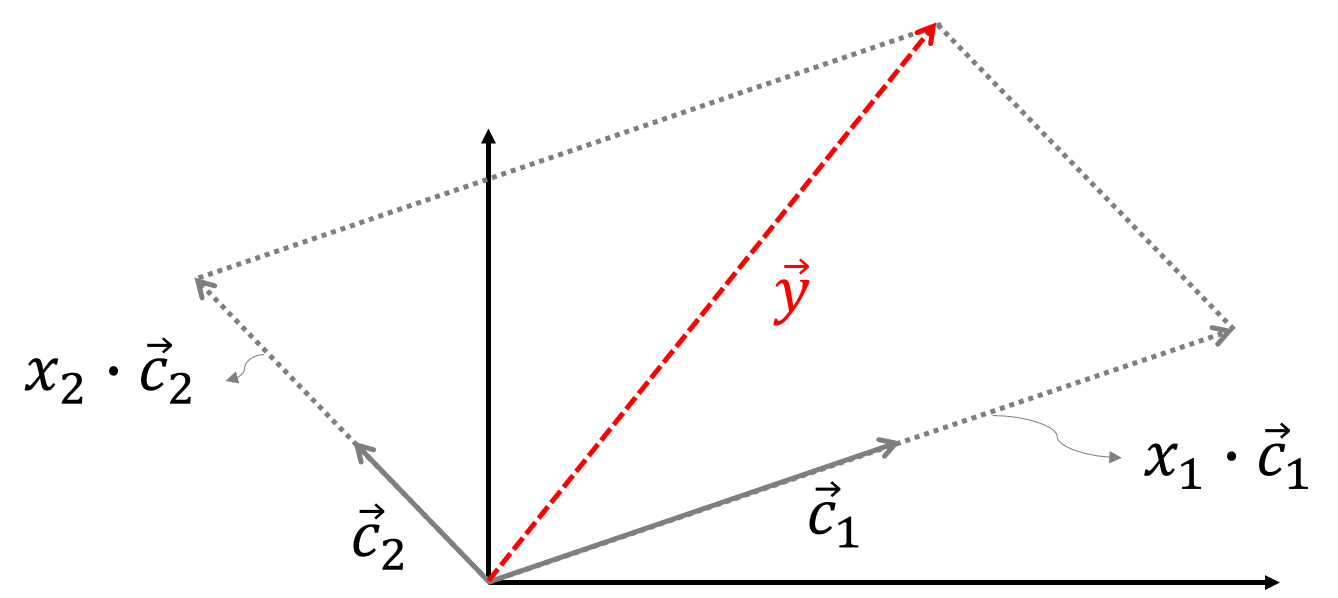
\includegraphics[width=0.60\textwidth]{lincomb.png}
	\caption{La multiplication matricielle comme une combinaison lineaire de vecteurs}
	\label{fig:lincomb}
\end{figure}
%%%%%%%%%%%%%%%%%%%%%%%%%%%%%%%%%%%%%%%%%%%%%%%%%%%%%%%%%%%%

De façon générale, le vecteur-colonne $\col{y}$ résultant d'une multiplication d'une matrice $A$ avec un vecteur-colonne $\col{x}$, peut-être exprimée comme une combinaison linéaire des colonnes de la matrice $A$:
%
\begin{align}
%
\left[ \begin{array}{c} 
	y_1 \\ \vdots \\ y_m
\end{array} \right] 
%
&= 
%
\left[ \begin{array}{c c c c c} 
\underbrace{\left[ \begin{array}{c} 
	a_{11} \\ \vdots \\ a_{1m}
\end{array} \right]}_{\col{c}_1}
& ... &
\underbrace{\left[ \begin{array}{c} 
	a_{i1} \\ \vdots \\ a_{im}
\end{array} \right]}_{\col{c}_i}
& ... &
\underbrace{\left[ \begin{array}{c} 
	a_{n1} \\ \vdots \\ a_{nm}
\end{array} \right]}_{\col{c}_n}
\end{array} \right] 
%
\left[ \begin{array}{c} 
	x_1 \\ \vdots \\ x_n
\end{array} \right]  \\
%
%
\col{y}
&= \sum_{i=1}^{n}{ \col{c}_i x_i}
\end{align}
%

%%%%%%%%%%%%%%%%%%%%%%%%%%%%%%%%%%%%%%%%%%%%%%%%%%%%%%%%%%
\section{Produits scalaires avec les rangés de la matrice} 
\label{sec:combveccol}
%%%%%%%%%%%%%%%%%%%%%%%%%%%%%%%%%%%%%%%%%%%%%%%%%%%%%%%%%%

Une autre interprétation de l'opération matricielle $\col{y} = A \col{x}$ est que chaque élément $y_j$ du résultat correspond au produit scalaire du vecteur-rangé $j$ avec le vecteur colonne $\col{x}$. L'équation \eqref{eq:sys2} peut prendre la forme:
%
\begin{align}
\left[ \begin{array}{c} 
	y_1 \\ y_2
\end{array} \right] &= 
\left[ \begin{array}{c c} 
a_{11} & a_{12} \\ a_{21} & a_{22}
\end{array} \right]
\left[ \begin{array}{c} 
	x_1 \\ x_2
\end{array} \right] = 
\left[ \begin{array}{c} 
\underbrace{
\left[ \begin{array}{c c} 
a_{11} & a_{12} 
\end{array} \right]
}_{\col{r}_1}
\left[ \begin{array}{c} 
	x_1 \\ x_2
\end{array} \right] 
	\\ \\
\underbrace{
\left[ \begin{array}{c c} 
a_{21} & a_{22} 
\end{array} \right]
}_{\col{r}_2}
\left[ \begin{array}{c} 
	x_1 \\ x_2
\end{array} \right] 
\end{array} \right] 
= 
\left[ \begin{array}{c} 
\vec{r}_1 \bullet \vec{x}
\\
\vec{r}_2 \bullet \vec{x}
\end{array} \right]
\end{align}
%
De façon générale, chaque élément du $y_j$ vecteur-colonne $\col{y}$ résultant d'une multiplication d'une matrice $A$ avec un vecteur-colonne $\col{x}$, peut-être exprimé comme le résultat du produit scalaire entre le vecteur-rangé $\col{r}_j$ et le vecteur-colonne $\col{x}$:
%
\begin{align}
y_j
&= \col{r}_j \, \col{x}
\end{align}
%


%%%%%%%%%%%%%%%%%%%%%%%%%%%%%%%%%%%%%%%%%%%%%%%%%%%%%%%%%%
\section{Opérations matricielles en termes d'indices et de composantes}
\label{sec:opmatind}
%%%%%%%%%%%%%%%%%%%%%%%%%%%%%%%%%%%%%%%%%%%%%%%%%%%%%%%%%%

Une matrice multipliée par un vecteur-colonne:

%%%%%%%%%%%%%%%%%%%%
\begin{align}
%%%%%%%%%%%%%%%%%%%%
\col{y}  = A \col{x} 
%%%%%%%%%%%%%%%%%%%%
\quad \Leftrightarrow \quad
%%%%%%%%%%%%%%%%%%%%
y_j = \sum_i{A_{ji} x_i }
%%%%%%%%%%%%%%%%%%%%
\end{align}
%%%%%%%%%%%%%%%%%%%%

Une matrice multipliée par une autre matrice:

%%%%%%%%%%%%%%%%%%%%
\begin{align}
%%%%%%%%%%%%%%%%%%%%
A  = B C
%%%%%%%%%%%%%%%%%%%%
\quad \Leftrightarrow \quad
%%%%%%%%%%%%%%%%%%%%
A_{ik} = \sum_j{B_{ij} C_{jk} }
%%%%%%%%%%%%%%%%%%%%
\end{align}
%%%%%%%%%%%%%%%%%%%%


%%%%%%%%%%%%%%%%%%%%%%%%%%%%%%%%%%%%%%%%%%%%%%%%%%%%%%%%%%
\section{Espace colonne}
\label{sec:espcol}
%%%%%%%%%%%%%%%%%%%%%%%%%%%%%%%%%%%%%%%%%%%%%%%%%%%%%%%%%%

L'espace colonne d'une matrice $A$ représente l'ensemble de toutes les valeurs possible de la sortie $\col{y}$ qui résulte de l'opération $\col{y} = A \col{x}$. Avec l'interprétation présentée à la section \ref{sec:combveccol}, il est possible de voir que cette sortie a comme domaine toutes les combinaisons linéaires possibles des vecteur-colonnes de la matrice. 

Par exemple, pour une matrice 3$\times$3 avec une sortie qui représente une position spatiale (x,y,z), dans le cas le plus générale la sortie peut potentiellement être une valeur arbitraire en 3D. Toutefois, si les vecteurs-colonnes de la matrice sont co-linéaire (donc  ils forment un plan), alors l'espace colonne est restreint à ce plan. La sortie $\col{y}$ peut seulement prendre des valeurs qui correspondent à ce plan. 

%%%%%%%%%%%%%%%%%%%%%%%%%%%%%%%%%%%%%%%%%%%%%%%%%%%%%%%%%%%%%
\begin{figure}[H]
	\centering
		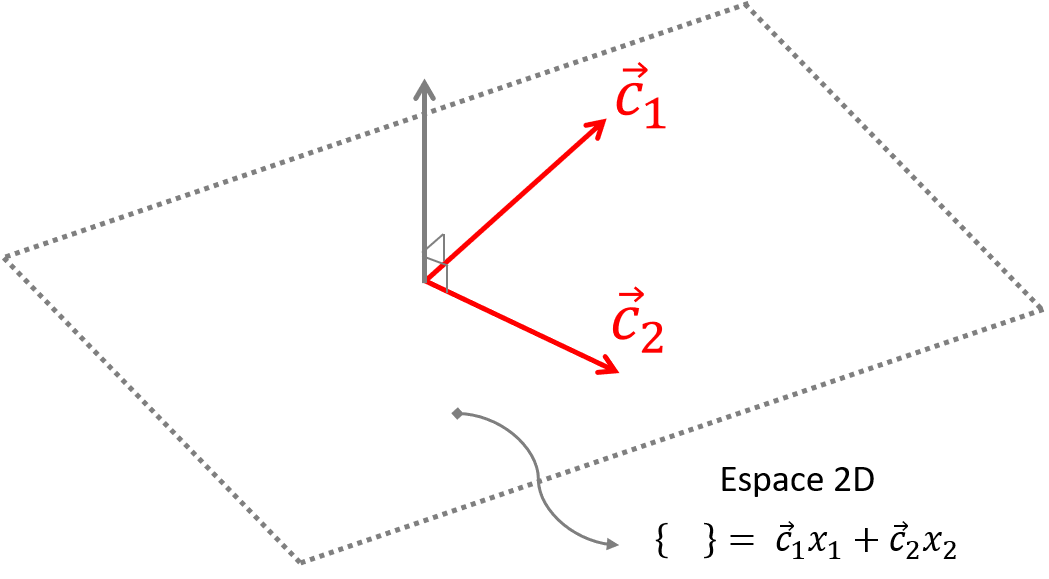
\includegraphics[width=0.60\textwidth]{2dspace.png}
	\caption{Visualisation graphique d'un espace colonne de dimension 2}
	\label{fig:2dspace}
\end{figure}
%%%%%%%%%%%%%%%%%%%%%%%%%%%%%%%%%%%%%%%%%%%%%%%%%%%%%%%%%%%%


L'espace colonne d'une matrice $A$ sera noté $col(A)$ et a la définition suivante:
%%%%%%%%%%%%%%%%%%%%%
\begin{align}
col(A) = 
\{ A \col{x} \; | \; \col{x} \in \re^n \}
\label{eq:cola}
\end{align}
%%%%%%%%%%%%%%%%%%%%%%

\textbf{Note sur la notation mathématique pour les ensembles:} Les crochets $\{ \}$ représentent un ensemble, à l'intérieur on note la liste des éléments de l'ensemble ou bien la définition. La barre verticale $|$ signifie \textit{tel que} et le symbole $\in$ signifie \textit{appartient à}. L'équation \eqref{eq:cola} peut donc se lire \textit{l'espace colonne de la matrice $A$ est égale à l'ensemble des résultats possible de l'opération $A \col{x} $ tel que $\col{x}$ appartient à l'espace vectoriel de dimension $n$}.

Lorsque la matrice $A$ est inversible, i.e. de rang plein, l'espace colonne correspond à $\re^m$, ou $m$ est le nombre de variables de sortie.

%%%%%%%%%%%%%%%%%%%%%%%%%%%%%%%%%%%%%%%%%%%%%%%%%%%%%%%%%%
\section{Espace rangée}
\label{sec:esprow}
%%%%%%%%%%%%%%%%%%%%%%%%%%%%%%%%%%%%%%%%%%%%%%%%%%%%%%%%%%

L'espace rangé d'une matrice correspond à l'ensemble des vecteur-colonne entré $\col{x}$ qui donne un vecteur-colonne sortie $\col{y}$ non-nul lorsque multiplié par la matrice $A$. Cet ensemble correspond aussi à toutes les combinaisons possibles des rangées de la matrice $A$.


L'espace rangée d'une matrice $A$ sera noté $row(A)$ et a la définition suivante:
%%%%%%%%%%%%%%%%%%%
\begin{align}
row(A) =  col(A^T) = 
\{ A^T \col{y} \; | \; \col{y} \in \re^m \}
\end{align}
%%%%%%%%%%%%%%%%%%%
Lorsque la matrice $A$ est inversible, i.e. de rang plein, l'espace rangé correspond à $\re^n$, ou $n$ est le nombre de variables de sortie.

%%%%%%%%%%%%%%%%%%%%%%%%%%%%%%%%%%%%%%%%%%%%%%%%%%%%%%%%%%
\section{Factorisation LU}
\label{sec:lu}
%%%%%%%%%%%%%%%%%%%%%%%%%%%%%%%%%%%%%%%%%%%%%%%%%%%%%%%%%%

Une matrice $A$ peut-etre factorise en deux matrices (triangulaires lorsque $A$ est une matrice inversible):
%
\begin{align}
A = LU 
\end{align}
%
ou la matrice $U$ est une matrice ou tout les coefficients sous la diagonale sont nuls et la matrice $L$ correspond aux opérations sur les ranges conduites dans le cadre d'une élimination Gauss-Jordan. Par exemple pour une matrice 3x3 inversible:
%
\begin{align}
L= 
\left[ \begin{array}{c c c } 
1      &   0       & 0   \\ 
l_{21} &   1       & 0   \\  
l_{31} & l_{32}    & 1
\end{array} \right]
\quad\quad
U = 
\left[ \begin{array}{c c c c c } 
p_{1} & u_{12} &  u_{13} \\ 
0     & p_{2}  &  u_{23}  \\ 
0     & 0      &  p_{3}
\end{array} \right]
\end{align}
%
Les coefficients non-nuls $p_i$ sur la diagonale de la matrice $U$ sont appeles les pivots.

%%%%%%%%%%%%%%%%%%%%%%%%%%%%%%%%%%%%%%%%%%%%%%%%%%%%%%%%%%
\section{Indépendance linéaire}
\label{sec:lindep}
%%%%%%%%%%%%%%%%%%%%%%%%%%%%%%%%%%%%%%%%%%%%%%%%%%%%%%%%%%

Un vecteur est dit linéairement dépendant d'un autre vecteur (ou un ensemble de vecteurs), lorsque celui-ci peut être exprimé comme un combinaison pondéré des autres. 

TODO figure

Un ensemble de vecteurs $\left\{ \col{v}_1, \col{v}_2, \hdots, \col{v}_n \right\}$ est \textbf{linéairement dépendant} s'il existe des coefficients non nuls $x_i$ tels que la somme pondérée des vecteurs est nulle:
%%%%%%%%%%%%%%%%%%%%%%
\begin{align}
\col{0} = x_1 \col{v}_1 + x_2 \col{v}_2 + ... + x_n \col{v}_n
\end{align}
%%%%%%%%%%%%%%%%%%%%%%%

Inversement, un ensemble de vecteurs $\left\{ \col{v}_1, \col{v}_2, \hdots, \col{v}_n \right\}$ est \textbf{linéairement indépendant} si:
%%%%%%%%%%%%%%%%%%%%%%
\begin{align}
\col{0} = x_1 \col{v}_1 + x_2 \col{v}_2 + ... + x_n \col{v}_n
\quad
\text{implique que:}
\quad
0 = x_1 = x_2 = ... = x_n 
\end{align}
%%%%%%%%%%%%%%%%%%%%%%%

%%%%%%%%%%%%%%%%%%%%%%%%%%%%%%%%%%%%%%%%%%%%%%%%%%%%%%%%%%
\section{Base}
\label{sec:base}
%%%%%%%%%%%%%%%%%%%%%%%%%%%%%%%%%%%%%%%%%%%%%%%%%%%%%%%%%%

Un ensemble $\{ \col{v}_1 \; \col{v}_2 \; \hdots \; \col{v}_n \}$ de vecteurs de dimensions $m$ dans un espace vectoriel appartenant à $\re^m$, forme une base de cet espace si: \textbf{1)} les vecteurs $\col{v}_1 \; \col{v}_2 \; \hdots \; \col{v}_n$ sont linéairement indépendants et \textbf{2)} tout vecteur $\col{w}$ de cet espace peut être exprimer comme une combinaison linéaire de ces vecteurs:
%%%%%%%%%%%%%%%%%%%%%%
\begin{align}
\col{w} = x_1 \col{v}_1 + x_2 \col{v}_2 + ... + x_n \col{v}_n
\end{align}
%%%%%%%%%%%%%%%%%%%%%%%

Par exemple, dans un espace tri-dimensionnel qui correspond à des coordonnées $
\left[
\begin{array}{c}
x \\ y \\ z
\end{array}
\right]
$, les vecteur-colonnes $\left\{ 
\left[
\begin{array}{c}
1 \\ 0 \\ 0
\end{array}
\right],
\left[
\begin{array}{c}
0 \\ 1 \\ 0
\end{array}
\right]
\right\}$
forment une base pour le sous-espace qui correspond au plan $z=0$.

%%%%%%%%%%%%%%%%%%%%%%%%%%%%%%%%%%%%%%%%%%%%%%%%%%%%%%%%%%
\section{Rang d'une matrice}
\label{sec:rang}
%%%%%%%%%%%%%%%%%%%%%%%%%%%%%%%%%%%%%%%%%%%%%%%%%%%%%%%%%%

Le rang $r$ d'une matrice correspond à la dimension de l'espace colonne d'une matrice, qui est toujours aussi égale à la dimension de l'espace rangé. Ce nombre correspond aussi au nombre de pivots, il sera noté par la variable $r$:
%%%%%%%%%%%%%%%%%%%%%%
\begin{align}
r = rank( A ) = dim( col(A) ) = dim( col(A^T) ) =\#\, pivots
\end{align}
%%%%%%%%%%%%%%%%%%%%%%%


Le rang d'une matrice est toujours inférieur ou égale aux dimensions $m$ et $n$.
%%%%%%%%%%%%%%%%%%%%%%%
\begin{align}
r \leq n &= \#\, ranges \\
r \leq m &= \#\, colonnes
\end{align}
%%%%%%%%%%%%%%%%%%%%%%%%

Dans le cas d'une matrice carré ($m=n$), il est possible de déterminer si la matrice à une rang dit plein, i.e. si $r=m=n$, en calculant le déterminant de la matrice $A$. Si le déterminant est non-nul alors la matrice à un rang plein.  

%%%%%%%%%%%%%%%%%%%%%%%%%%%%%%%%%%%%%%%%%%%%%%%%%%%%%%%%%%
\section{Rang plein vs. Trop de variables vs. Trop d’équations}
\label{sec:rangpleinvstrop}
%%%%%%%%%%%%%%%%%%%%%%%%%%%%%%%%%%%%%%%%%%%%%%%%%%%%%%%%%%

Un système d'équations peut être parfaitement contraint (une seule solution existe), sur-contraint (aucune solution exacte n'existe) ou bien sous-contraint (plusieurs solutions sont possible. Dans le cas d'une relation matricielle de type $A \col{x} = \col{y} $, qui représente un système d’équations linéaires, le rang de la matrice $A$ permet de déterminer la situation, voir figure \ref{fig:rmn}.

%%%%%%%%%%%%%%%%%%%%%%%%%%%%%%%%%%%%%%%%%%%%%%%%%%%%%%%%%%%%%
\begin{figure}[htp]
	\centering
		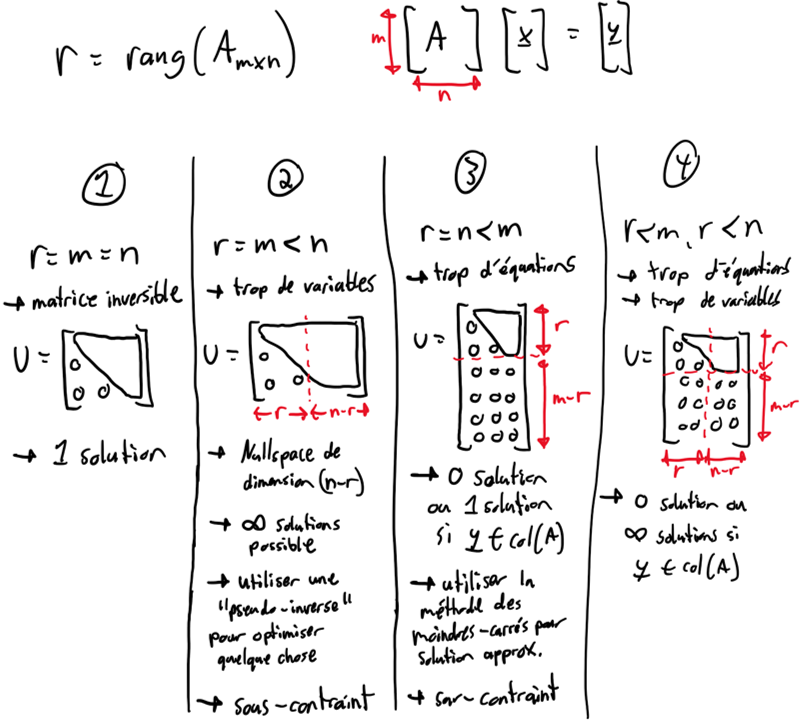
\includegraphics[width=0.95\textwidth]{linalgebra_4types.png}
	\caption{Quatre situations possibles pour un système d'équations}
	\label{fig:rmn}
\end{figure}
%%%%%%%%%%%%%%%%%%%%%%%%%%%%%%%%%%%%%%%%%%%%%%%%%%%%%%%%%%%%

Les grandes catégories de situations possibles illustrés à la figure \ref{fig:rmn} sont exemplifiés avec les exemples illustrés aux figures \ref{fig:rmn_ex1}, \ref{fig:rmn_ex2}, \ref{fig:rmn_ex3} et \ref{fig:rmn_ex4}.

%%%%%%%%%%%%%%%%%%%%%%%%%%%%%%%%%%%%%%%%%%%%%%%%%%%%%%%%%%%%%
\begin{figure}[htp]
	\centering
		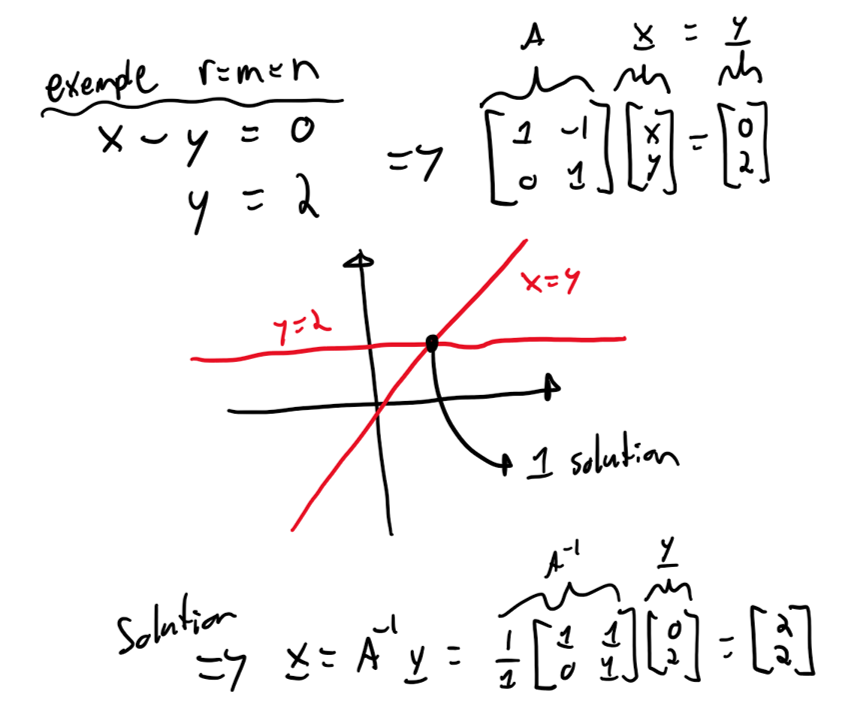
\includegraphics[width=0.65\textwidth]{linalgebra_4types_ex1.png}
	\caption{Exemple d'un système d'équation parfaitement contraint}
	\label{fig:rmn_ex1}
\end{figure}
%%%%%%%%%%%%%%%%%%%%%%%%%%%%%%%%%%%%%%%%%%%%%%%%%%%%%%%%%%%%

%%%%%%%%%%%%%%%%%%%%%%%%%%%%%%%%%%%%%%%%%%%%%%%%%%%%%%%%%%%
\begin{figure}[htp]
	\centering
		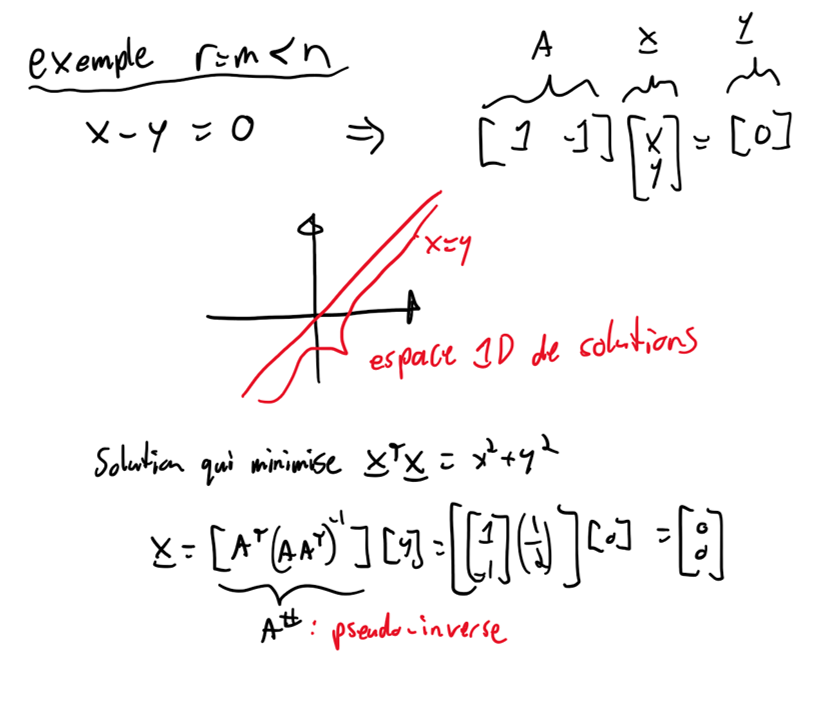
\includegraphics[width=0.65\textwidth]{linalgebra_4types_ex2.png}
	\caption{Exemple d'un système d'équation sous-contraint}
	\label{fig:rmn_ex2}
\end{figure}
%%%%%%%%%%%%%%%%%%%%%%%%%%%%%%%%%%%%%%%%%%%%%%%%%%%%%%%%%%%%

%%%%%%%%%%%%%%%%%%%%%%%%%%%%%%%%%%%%%%%%%%%%%%%%%%%%%%%%%%%%
\begin{figure}[htp]
	\centering
		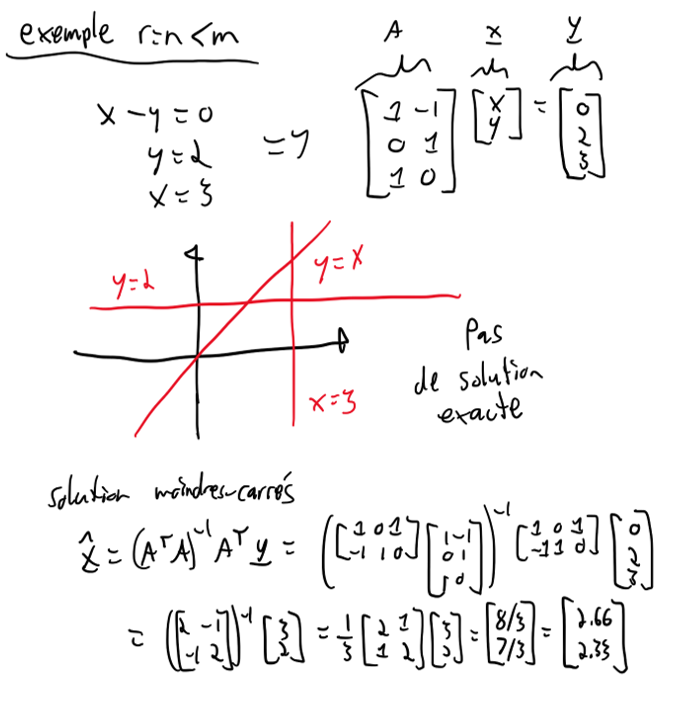
\includegraphics[width=0.65\textwidth]{linalgebra_4types_ex3.png}
	\caption{Exemple d'un système d'équation sur-contraint}
	\label{fig:rmn_ex3}
\end{figure}
%%%%%%%%%%%%%%%%%%%%%%%%%%%%%%%%%%%%%%%%%%%%%%%%%%%%%%%%%%%%%

%%%%%%%%%%%%%%%%%%%%%%%%%%%%%%%%%%%%%%%%%%%%%%%%%%%%%%%%%%%%%
\begin{figure}[htp]
	\centering
		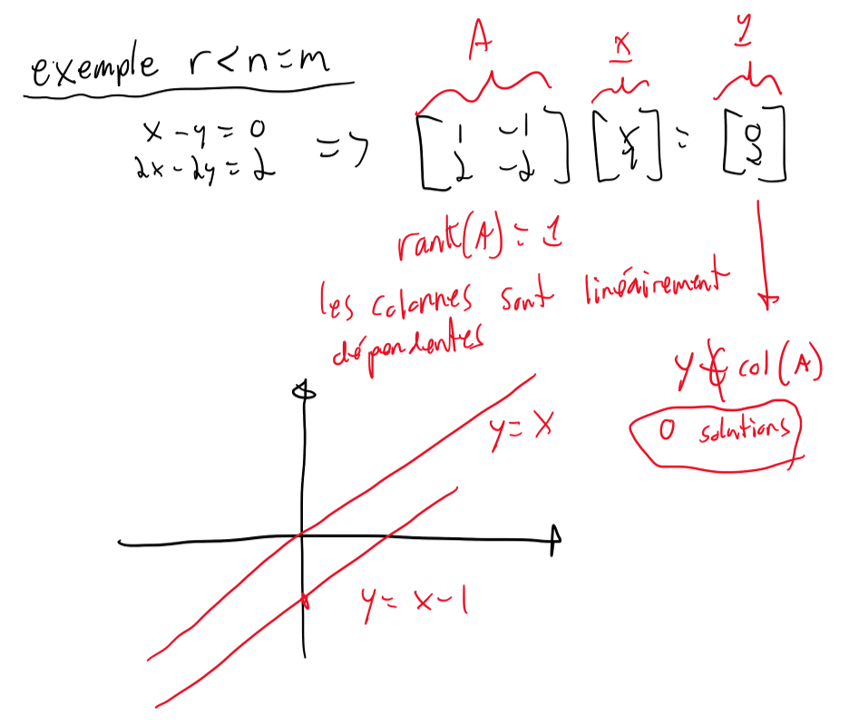
\includegraphics[width=0.65\textwidth]{linalgebra_4types_ex4.png}
	\caption{Exemple d'un système d'équation non-inversible}
	\label{fig:rmn_ex4}
\end{figure}
%%%%%%%%%%%%%%%%%%%%%%%%%%%%%%%%%%%%%%%%%%%%%%%%%%%%%%%%%%%%%


%%%%%%%%%%%%%%%%%%%%%%%%%%%%%%%%%%%%%%%%%%%%%%%%%%%%%%%%%%
\newpage
\section{Nullspace}
\label{sec:nullspace}
%%%%%%%%%%%%%%%%%%%%%%%%%%%%%%%%%%%%%%%%%%%%%%%%%%%%%%%%%%

Le \textit{Nullspace} d'une matrice $A$, noté $N(A)$ correspond a l'ensemble de tous les vecteur-colonnes $\col{x}$ pour lesquels la multiplication avec la matrice $A$ donne un vecteur-colonne nulle $\col{0}$ :
%%%%%%%%%%%%%%%%%%%%%%%%%%%
\begin{align}
N(A) = \left\{ \col{x} \in \mathbb{R}^n \,|\, A\col{x} = \col{0} \right\}
\end{align}
%%%%%%%%%%%%%%%%%%%%%%%%%%%

Tous les vecteur-colonnes entrées $\col{x}$ pour une matrice appartiennent soit à l'espace rangé soit au \textit{Nullspace}:
%%%%%%%%%%%%%%%%%%%%%%%%%%%
\begin{align}
\col{x} \in \re^n = col(A^T) \; \cup \; N(A) %\quad \text{et} \quad
%n     = dim( row(A) ) + dim( N(A) ) 
\end{align}
%%%%%%%%%%%%%%%%%%%%%%%%%%%

\textbf{Les vecteur-colonnes appartenant à l'espace rangé influencent la sortie alors que les vecteur-colonnes appartenant au \textit{Nullspace} n'influent pas la sortie.} 

Une matrice $A$ va avoir un \textit{Nullspace} seulement lorsqu'elle a une rang déficient, donc des colonnes linéairement dépendantes. La présence d'un \textit{Nullspace} indique un système sous-contraint ou il y a un surplus de variables, donc plusieurs solutions possibles d'entrées $\col{x}$ pour obtenir une même sortie $\col{y}$. 
%
%\textbf{Utilisation} Une utilité du \textit{Nullspace} est que si on connaît un solution $\col{x}_s$ tel que: 
%%%%%%%%%%%%%%%%%%%%%%%%%%%%
%\begin{align}
%A \col{x}_s = \col{y}
%\end{align}
%%%%%%%%%%%%%%%%%%%%%%%%%%%%
%Il est possible de trouver les autres solutions possible directement si on connaît le \textit{Nullspace}, car une addition de la solution connue et d'un vecteur-colonne appartenant au \textit{Nullspace} ($\col{x}_n \in N(A) $)  est aussi une solution: 
%%%%%%%%%%%%%%%%%%%%%%%%%%%%
%\begin{align}
%A ( \col{x}_s + \col{x}_n) = A \col{x}_s + 
%\underbrace{
%A \col{x}_n 
%}_{ \col{0} }
%= A \col{x}_s = \col{y}
%\end{align}
%%%%%%%%%%%%%%%%%%%%%%%%%%%%
%
La figure \ref{fig:4spaces_ex1} illustre la signification physique du \textit{Nullspace} d'une matrice qui relie la vitesse des joints d'un robot manipulateur à la vitesse de son effecteur. 

%%%%%%%%%%%%%%%%%%%%%%%%%%%%%%%%%%%%%%%%%%%%%%%%%%%%%%%%%%
\section{Left-Nullspace}
\label{sec:leftnullspace}
%%%%%%%%%%%%%%%%%%%%%%%%%%%%%%%%%%%%%%%%%%%%%%%%%%%%%%%%%%

Le \textit{Left-Nullspace} d'une matrice $A$, noté $N(A^T)$ correspond a l'ensemble de tous les vecteur-colonnes $\col{y}$ pour lesquels la multiplication avec la matrice $A^T$ donne un vecteur-colonne nulle $\col{0}$ :
%%%%%%%%%%%%%%%%%%%%%%%%%%%
\begin{align}
N(A^T) = \left\{ \col{y} \in \mathbb{R}^m \,|\, A^T\col{y} = \col{0} \right\}
\end{align}
%%%%%%%%%%%%%%%%%%%%%%%%%%%

Tous les vecteur-colonnes sorties $\col{y}$ appartiennent soit à l'espace colonne soit au \textit{Left-Nullspace}:
%%%%%%%%%%%%%%%%%%%%%%%%%%%
\begin{align}
\col{y} \in \re^m = col(A) \; \cup \; N(A^T) %\quad \text{et} \quad
%n     = dim( row(A) ) + dim( N(A) ) 
\end{align}
%%%%%%%%%%%%%%%%%%%%%%%%%%%

\textbf{Les vecteur-colonnes $\col{y}$ appartenant à l'espace colonne ont une solution $\col{x}$ possible, tandis que ceux appartenant au \textit{Left-Nullspace} n'ont aucune solution exacte $\col{x}$ possible}.

Une matrice $A$ va avoir un \textit{Left-Nullspace} seulement lorsqu'elle a une rang déficient. La présence d'un \textit{Left-Nullspace} indique un système sur-contraint ou il y a un surplus d'équations, donc plusieurs sortie $\col{y}$ pour lesquels il n'y a pas de solutions $\col{x}$.


%%%%%%%%%%%%%%%%%%%%%%%%%%%%%%%%%%%%%%%%%%%%%%%%%%%%%%%%%%
\section{Les quatre espaces fondamentaux}
\label{sec:4espfond}
%%%%%%%%%%%%%%%%%%%%%%%%%%%%%%%%%%%%%%%%%%%%%%%%%%%%%%%%%%

La figure \ref{fig:4spaces} résume les quatre espaces fondamentaux d'une matrice, deux sont caractérisent les entrées et deux espaces caractérisent les sorties. La figure \ref{fig:4spaces2} illustre comment les dimensions de ces espaces sont reliés au rang et dimensions d'une matrice.

%%%%%%%%%%%%%%%%%%%%%%%%%%%%%%%%%%%%%%%%%%%%%%%%%%%%%%%%%%%%%
\begin{figure}[H]
	\centering
		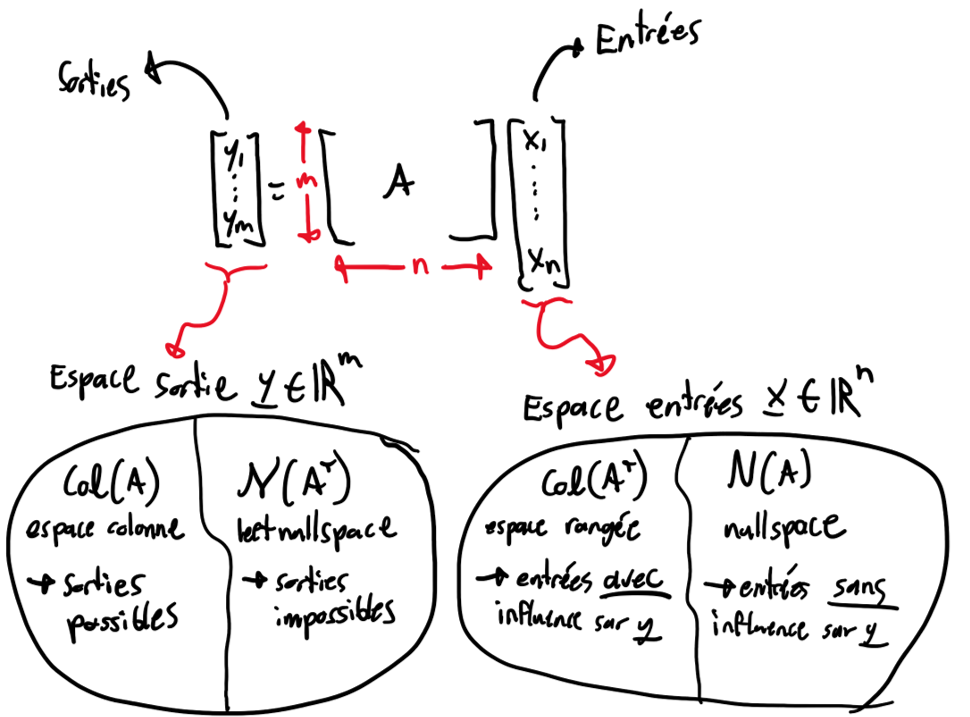
\includegraphics[width=0.85\textwidth]{linalgebra_4spaces.png}
	\caption{Quatres espaces fondamentaux d'une matrice}
	\label{fig:4spaces}
\end{figure}
%%%%%%%%%%%%%%%%%%%%%%%%%%%%%%%%%%%%%%%%%%%%%%%%%%%%%%%%%%%%%

%%%%%%%%%%%%%%%%%%%%%%%%%%%%%%%%%%%%%%%%%%%%%%%%%%%%%%%%%%%%
\begin{figure}[H]
	\centering
		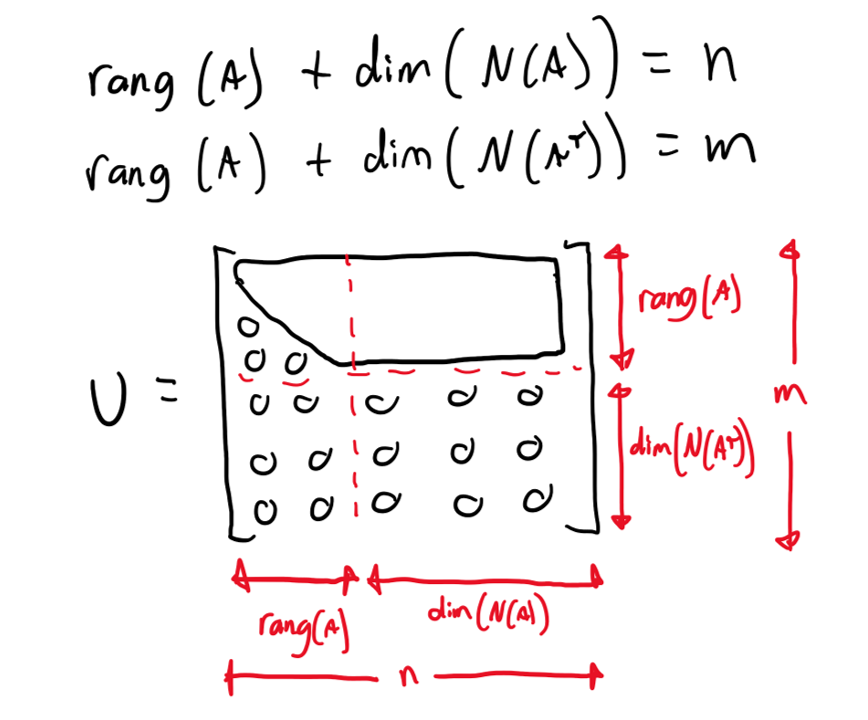
\includegraphics[width=0.60\textwidth]{linalgebra_4spaces2.png}
	\caption{Dimensions des quatre espaces fondamentaux d'une matrice}
	\label{fig:4spaces2}
\end{figure}
%%%%%%%%%%%%%%%%%%%%%%%%%%%%%%%%%%%%%%%%%%%%%%%%%%%%%%%%%%%%

%%%%%%%%%%%%%%%%%%%%%%%%%%%%%%%%%%%%%%%%%%%%%%%%%%%%%%%%%%%%
\begin{figure}[H]
	\centering
		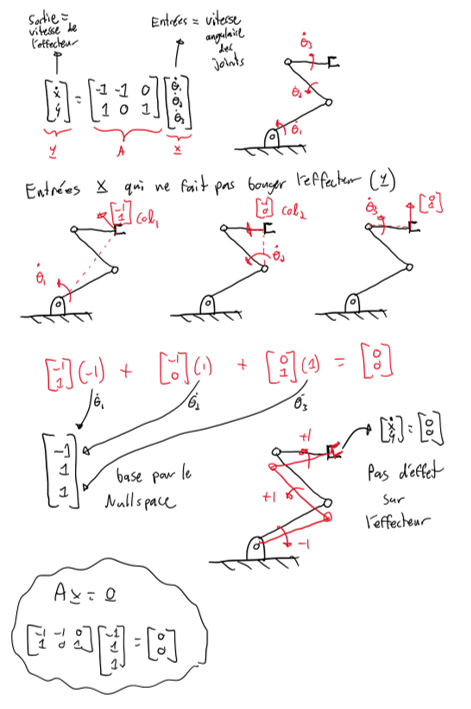
\includegraphics[width=0.85\textwidth]{linalgebra_4spaces_ex1.png}
	\caption{Exemple de Nullspace d'une matrice}
	\label{fig:4spaces_ex1}
\end{figure}
%%%%%%%%%%%%%%%%%%%%%%%%%%%%%%%%%%%%%%%%%%%%%%%%%%%%%%%%%%%%

%%%%%%%%%%%%%%%%%%%%%%%%%%%%%%%%%%%%%%%%%%%%%%%%%%%%%%%%%%%%
\begin{figure}[H]
	\centering
		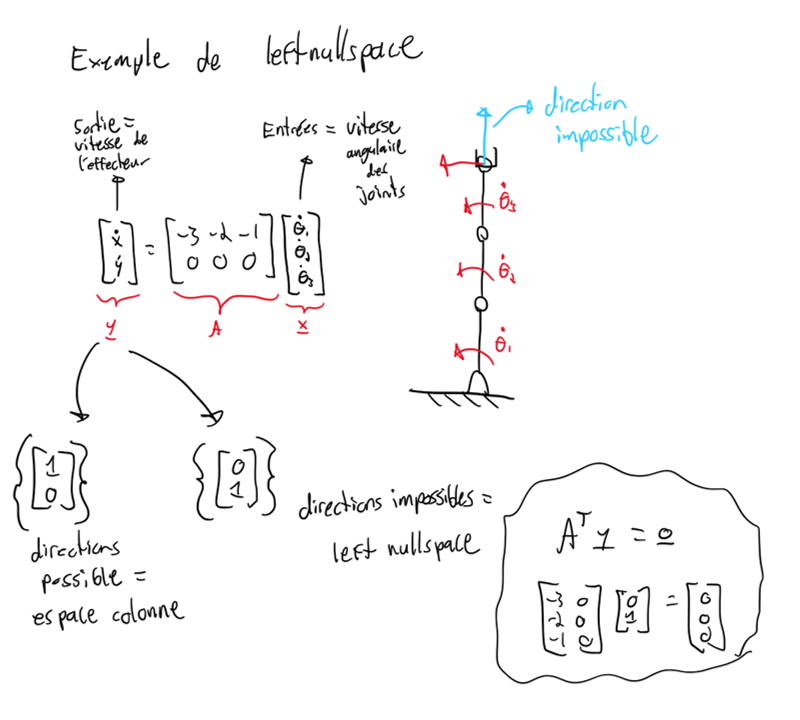
\includegraphics[width=0.85\textwidth]{linalgebra_4spaces_ex2.png}
	\caption{Exemple de Left-Nullspace d'une matrice}
	\label{fig:4spaces_ex2}
\end{figure}
%%%%%%%%%%%%%%%%%%%%%%%%%%%%%%%%%%%%%%%%%%%%%%%%%%%%%%%%%%%%


%%%%%%%%%%%%%%%%%%%%%%%%%%%%%%%%%%%%%%%%%%%%%%%%%%%%%%%%%%%%
\section{Projection}
%%%%%%%%%%%%%%%%%%%%%%%%%%%%%%%%%%%%%%%%%%%%%%%%%%%%%%%%%%%%

À venir!

%%%%%%%%%%%%%%%%%%%%%%%%%%%%%%%%%%%%%%%%%%%%%%%%%%%%%%%%%%%%
\section{Moindres carrés}
%%%%%%%%%%%%%%%%%%%%%%%%%%%%%%%%%%%%%%%%%%%%%%%%%%%%%%%%%%%%

À venir!

%%%%%%%%%%%%%%%%%%%%%%%%%%%%%%%%%%%%%%%%%%%%%%%%%%%%%%%%%%%%
\section{Pseudo-Inverse}
%%%%%%%%%%%%%%%%%%%%%%%%%%%%%%%%%%%%%%%%%%%%%%%%%%%%%%%%%%%%

À venir!


%%%%%%%%%%%%%%%%%%%%%%%%%%%%%%%%%%%%%%%%%%%%%%%%%%%%%%%%%%%%%
\newpage
\section{Graphical Interpretation of the Least Square Solution}

Given an input-output model with linearly involved parameters:
\begin{align}
\underline{\varphi}^T \underline{\theta}
= y
\quad\quad\Rightarrow\quad\quad
\underbrace{ 
\left[ \begin{array}{c c c } 
\varphi_1 & ... & \varphi_m
\end{array} \right] }_{ m \text{ known inputs} }
\underbrace{ \left[ \begin{array}{c} 
\theta_1 \\ \vdots \\ \theta_m
\end{array} \right] }_{ m \text{ unknown parameters} } = 
\underbrace{y}_{\text{known scalar output} }
\end{align}

Given an $N$ samples of input-output data:
\begin{align}
\Phi^T \underline{\theta}
= \underline{y}
\quad\quad\Rightarrow\quad\quad
\underbrace{ 
\left[ \begin{array}{c c c c c } 
&& \underline{\varphi}^T(1) && \\
&& \vdots & \\
&& \underline{\varphi}^T(N) && \\
\end{array} \right] }_{\text{ $\Phi^T$ : $N \times m$  inputs data} }
\left[ \begin{array}{c} 
\theta_1 \\ \vdots \\ \theta_m
\end{array} \right]
 = \underbrace{ \left[ \begin{array}{c}  
 y(1) \\ \vdots \\ y(N)\\ 
 \end{array} \right] }_{ \text{ $\underline{y}$: $N$ output samples} } 
\end{align}

Column of matrix $\Phi^T$ span a $N$ dimension hyperplane:
%%%%%%%%%%%%%%%%%%%%%%%%%%%%%%%%%%%%%%%%%%%%%%%%%%%%%%%
\begin{align}
\Phi^T = 
\left[ \begin{array}{c@{}c@{}c}  
\left[  \begin{array}{c}  \\ \underline{c_1} \\ \\ \end{array} \right] &  \ldots & \left[  \begin{array}{c} \\ \underline{c_m} \\ \\ \end{array} \right]
\end{array} \right]
\end{align}
%%%%%%%%%%%%%%%%%%%%%%%%%%%%%%%%%%%%%%%%%%%%%%%%%%%%%%%%%%

Exact solution does not exist when $\underline{y} \notin col( \Phi^T )$, instead we look for an approximation:
\begin{align}
\text{Projection Approximation : }
\Phi^T \hat{\underline{\theta}}= \underline{p}
\quad\quad\quad
\text{Error : }
\underline{e} = \underline{y} - \underline{p}
\end{align}
The distance between the approximation $\underline{p}$ and $\underline{y}$ is minimal when the error $\underline{e}$ is orthogonal to the column space hyperplane:
\begin{align}
\underline{c}_i^T \underline{e}= 0 \quad \forall \, i
\quad\Rightarrow\quad
\Phi \underline{e}= \underline{0}
\quad\Rightarrow\quad
\Phi ( \, \underline{y} - \Phi^T \hat{\underline{\theta}} \, )= \underline{0}
\quad\Rightarrow\quad
\hat{\underline{\theta}} = \left[ \Phi \Phi^T \right]^{-1} \Phi \underline{y}
\end{align}

\begin{figure}[htp]
	\centering
		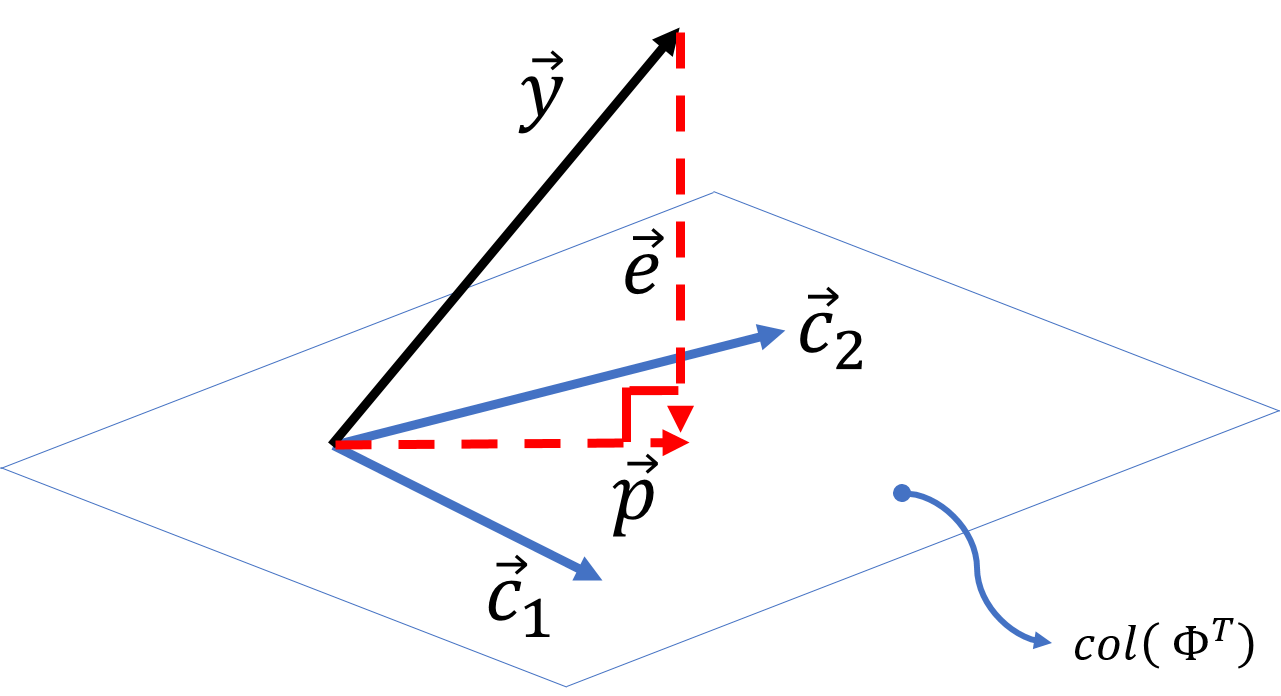
\includegraphics[width=0.45\textwidth]{projectionLS.png}
	\caption{Graphical Visualization of Least Square}
\end{figure}


%%%%%%%%%%%%%%%%%%%%%%%%%%%%%%%%%%%%%%%%%%%%%%%%%%%%%%%%%%%%
\section{Base orthonormale}
%%%%%%%%%%%%%%%%%%%%%%%%%%%%%%%%%%%%%%%%%%%%%%%%%%%%%%%%%%%%

À venir!

%%%%%%%%%%%%%%%%%%%%%%%%%%%%%%%%%%%%%%%%%%%%%%%%%%%%%%%%%%%%
\section{Déterminants}
%%%%%%%%%%%%%%%%%%%%%%%%%%%%%%%%%%%%%%%%%%%%%%%%%%%%%%%%%%%%



%%%%%%%%%%%%%%%%%%%%%%%%
\begin{align}
det(A) = det(U) = p_1 p_2 ... p_n
\end{align}
%%%%%%%%%%%%%%%%%%%%%%%%

%%%%%%%%%%%%%%%%%%%%%%%%%%%%%%%%%%%%%%%%%%%%%%%%%%%%%%%%%%%%
\section{Vecteurs et valeurs propres (eigen values/vectors)}
%%%%%%%%%%%%%%%%%%%%%%%%%%%%%%%%%%%%%%%%%%%%%%%%%%%%%%%%%%%%

Pour les matrices carrées ($m=n$), une autre caractéristique utile est l'ensemble de ses vecteurs et valeurs propres. Un vecteur $\col{x}$ est un vecteur propre d'une matrice $A$ si le résultat $\col{y} = A \col{x}$ est parallèle à l'entrée $\col{x}$, autrement dit s'il existe un scalaire $\lambda$ (appelé valeur propre) tel que:
%%%%%%%%%%%%%%%%%%%%%%%%%%%
\begin{align}
A \col{x} = \lambda  \col{x}
\end{align}
%%%%%%%%%%%%%%%%%%%%%%%%%%%

%%%%%%%%%%%%%%%%%%%%%%%%%%%%%%%%%%%%%%%%%%%%%%%%%%%%%%%%%%%%%
\begin{figure}[H]
	\centering
		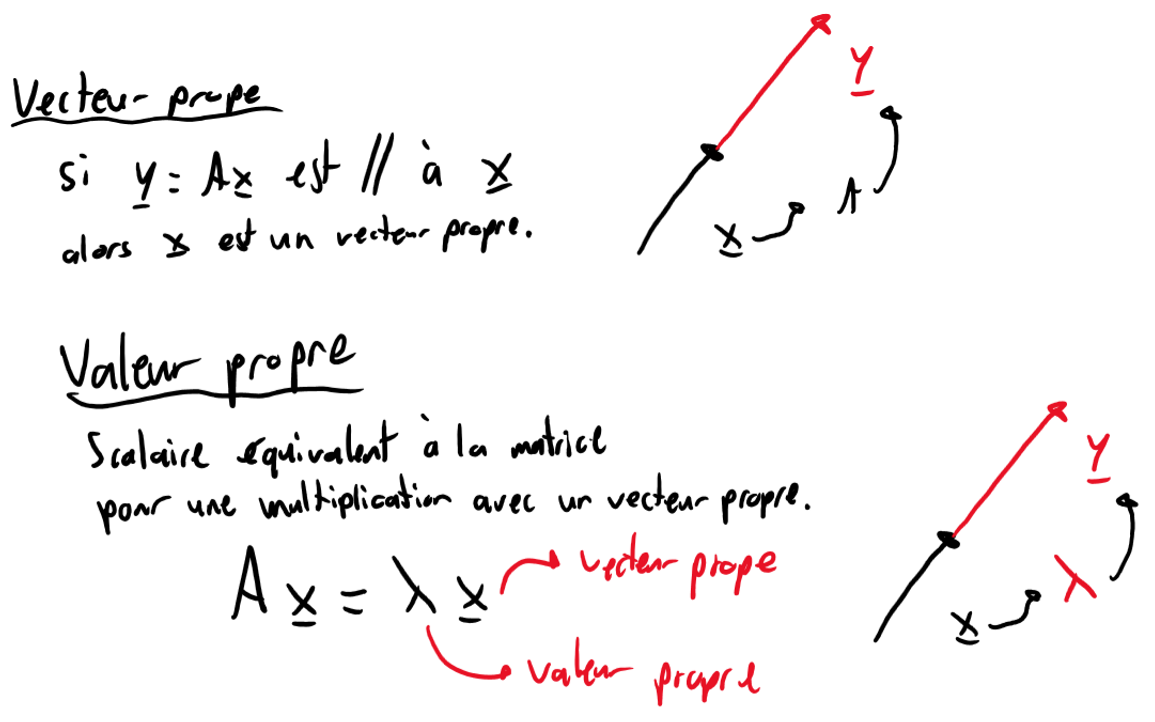
\includegraphics[width=0.85\textwidth]{linalgebra_eigen.png}
	\caption{Vecteurs et valeurs propres}
	\label{fig:eigen}
\end{figure}
%%%%%%%%%%%%%%%%%%%%%%%%%%%%%%%%%%%%%%%%%%%%%%%%%%%%%%%%%%%%%

Un matrice $n \times n$ va avoir $n$ paires de vecteur et valeurs propres (qui peuvent être répété et aussi des nombres complexes). Si une ou plusieurs valeurs propres de la matrice est égale à zéro alors la matrice est singulière et les vecteurs propres associés forme une base du nullspace de la matrice. 

La trace d'un matrice est égale à la somme des valeurs propres et le déterminant d'une matrice est égale à la multiplication de toutes les valeurs propres:
%%%%%%%%%%%%%%%%%%%%%%%%%%%
\begin{align}
trace(A) &= \sum_1^n{ \lambda_i } \\
det(A)   &= \prod_1^n{ \lambda_i }
\end{align}
%%%%%%%%%%%%%%%%%%%%%%%%%%%

Pour déterminer les valeurs et vecteurs propres d'une matrice, le problème est posé ainsi:
%%%%%%%%%%%%%%%%%%%%%%%%%%%
\begin{align}
A \col{x} &= \lambda  \col{x} \\
(A - \lambda I) \col{x} &= \col{0}
\end{align}
%%%%%%%%%%%%%%%%%%%%%%%%%%%
La matrice $(A - \lambda I)$ doit être singulière pour qu'il existe des solutions non-nulles à cette équation. Il est donc possible de trouver les valeurs propres $\lambda_i$ en solutionnant l'équation suivante:
%%%%%%%%%%%%%%%%%%%%%%%%%%%
\begin{align}
det(A - \lambda I) = 0
\end{align}
%%%%%%%%%%%%%%%%%%%%%%%%%%%
Pour chaque solution, i.e pour chaque valeur propre $\lambda_i$, il est possible de déterminer le vecteur propre associé $\col{v}_i$ en déterminant le nullspace de $(A - \lambda I)$:
%%%%%%%%%%%%%%%%%%%%%%%%%%%
\begin{align}
\col{v}_i \in nullspace(A - \lambda I)
\end{align}
%%%%%%%%%%%%%%%%%%%%%%%%%%%
Il est à noté que pour chaque valeur propre, le vecteur propre n'est pas unique, seule la direction l'est. Si $\col{v}_i$ est un vecteur propre alors tout multiple de lui même est aussi un vecteur propre. Donc autrement dit pour chaque valeur propre $\lambda_i$, on cherche en fait une base pour l'espace 1D associé aux vecteurs propres de cette valeur.



%%%%%%%%%%%%%%%%%%%%%%%%%%%%%%%%%%%%%%%%%%%%%%%%%%%%%%%%%%%%%
\begin{figure}[H]
	\centering
		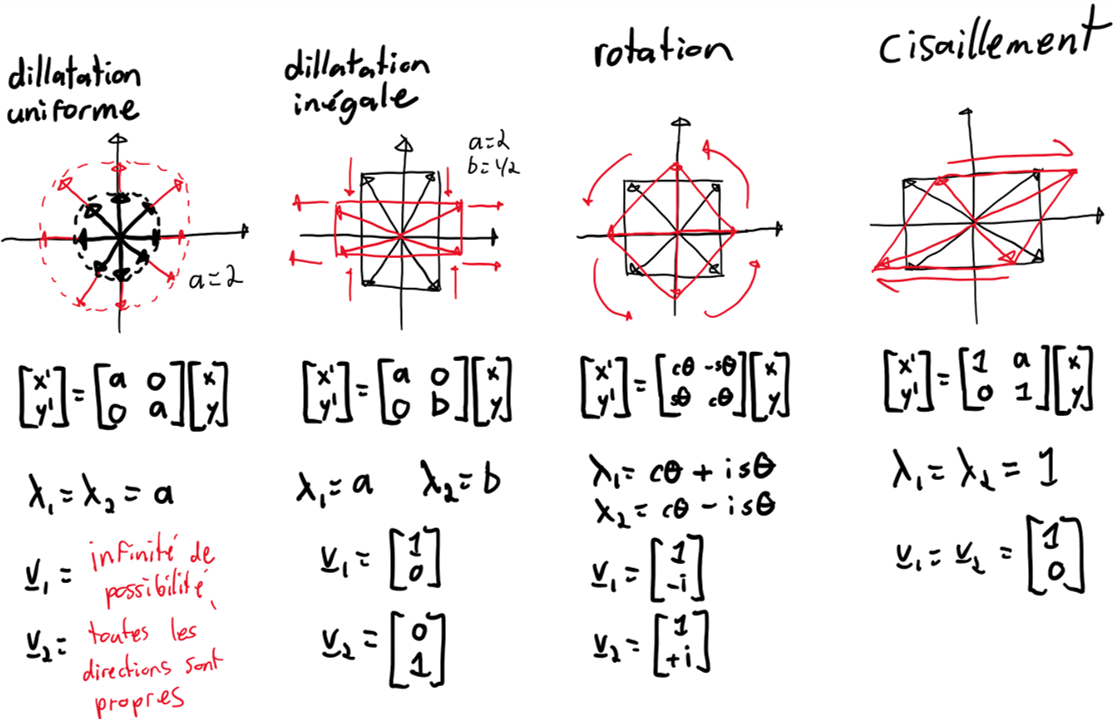
\includegraphics[width=0.95\textwidth]{linalgebra_eigen_exemple.png}
	\caption{Exemple de vecteurs et valeurs propres dans un contexte de transformations géométriques}
	\label{fig:linalgebra_eigen_exemple}
\end{figure}
%%%%%%%%%%%%%%%%%%%%%%%%%%%%%%%%%%%%%%%%%%%%%%%%%%%%%%%%%%%%%

%%%%%%%%%%%%%%%%%%%%%%%%%%%%%%%%%%%%%%%%%%%%%%%%%%%%%%%%%%%%
\section{Diagonalisation}
%%%%%%%%%%%%%%%%%%%%%%%%%%%%%%%%%%%%%%%%%%%%%%%%%%%%%%%%%%%%

Si une matrice a $n$ vecteurs propres indépendants, alors la matrice peut être diagonalisée, c'est à dire décomposée sous la forme:
%%%%%%%%%%%%%%%%%%%%%%%%%%%
\begin{align}
A = V \Lambda V^{-1}
\label{eq:diagmatrix}
\end{align}
%%%%%%%%%%%%%%%%%%%%%%%%%%%
où la matrice $V$ regroupe tous les vecteurs propres de $A$, et la matrice diagonale $\Lambda$ toutes les valeurs propres  de $A$:
%%%%%%%%%%%%%%%%%%%%%%%%%%%
\begin{align}
V = 
\left[ \begin{array}{c@{}c@{}c}  
\left[  \begin{array}{c}  \\ \underline{v}_1 \\ \\ \end{array} \right] &  \ldots & \left[  \begin{array}{c} \\ \underline{v}_n \\ \\ \end{array} \right]
\end{array} \right]
\quad \quad
\Lambda = 
\left[ \begin{array}{c c c c}  
\lambda_1 &  0          & 0 & 0 \\
0         &  \lambda_2  & 0      & 0 \\
0         &  0          &\ddots  & 0 \\
0         &  0          & 0  & \lambda_n
\end{array} \right]
\end{align}
%%%%%%%%%%%%%%%%%%%%%%%%%%%

Lorsqu'une matrice a plusieurs vecteur propres associés à la même valeur propre alors la matrice n'est pas diagonalisable. Il est toutefois possible de faire appelle à une méthode alternative appelée la réduction de Jordan. 
%
La diagonalisation d'une matrice peut être interprété comme un changement de base, vers des coordonnées dites propres, pour lesquelles l'effet de la multiplication de cette matrice est indépendant pour chaque axes. 


%%%%%%%%%%%%%%%%%%%%%%%%%%%%%%%%%%%%%%%%%%%%%
\subsection{Preuve}
\label{sec:preuvediag}
%%%%%%%%%%%%%%%%%%%%%%%%%%%%%%%%%%%%%%%%%%%%%

Par définition, si les vecteurs propres $\col{v}_i$ sont multipliés leur matrice $A$, la multiplication est équivalente à les multiplier par les valeurs propres associées $\lambda_i$:
%
%%%%%%%%%%%%%%%%%%%%%%%%%%%
\begin{align}
A V = 
\left[ \begin{array}{c@{}c@{}c}  
A \left[   \begin{array}{c}  \\ \underline{v}_1 \\ \\ \end{array} \right] &  \ldots & \; A \left[  \begin{array}{c} \\ \underline{v}_n \\ \\ \end{array} \right]
\end{array} \right]
= 
\left[ \begin{array}{c@{}c@{}c}  
\lambda_1 \left[   \begin{array}{c}  \\ \underline{v}_1 \\ \\ \end{array} \right] &  \ldots & \;\lambda_n \left[  \begin{array}{c} \\  \underline{v}_n \\ \\ \end{array} \right]
\end{array} \right]
= V \Lambda
\end{align}
\label{eq:diagproof}
%%%%%%%%%%%%%%%%%%%%%%%%%%%
Ensuite, si la matrice $V$ est inversible (ce qui explique la condition d'indépendance des vecteurs propres pour que la matrice soit diagonalisable), il suffit de multiplier l'équation \eqref{eq:diagmatrix} par $V^{-1}$ par la droite pour obtenir l'équation \eqref{eq:diagmatrix}. 




%%%%%%%%%%%%%%%%%%%%%%%%%%%%%%%%%%%%%%%%%%%%%%%%%%%%%%
\subsection{Exemple de diagonalisation pour une dillatation en 2D}
\label{sec:ExempleDeDiagonalisationPourUneDillatationEn2D}
%%%%%%%%%%%%%%%%%%%%%%%%%%%%%%%%%%%%%%%%%%%%%%%%%%%%%%

%%%%%%%%%%%%%%%%%%%%%%%%%%%%%%%%%%%%%%%%%%%%%%%%%%%%%%%%%%%%%
\begin{figure}[H]
	\centering
		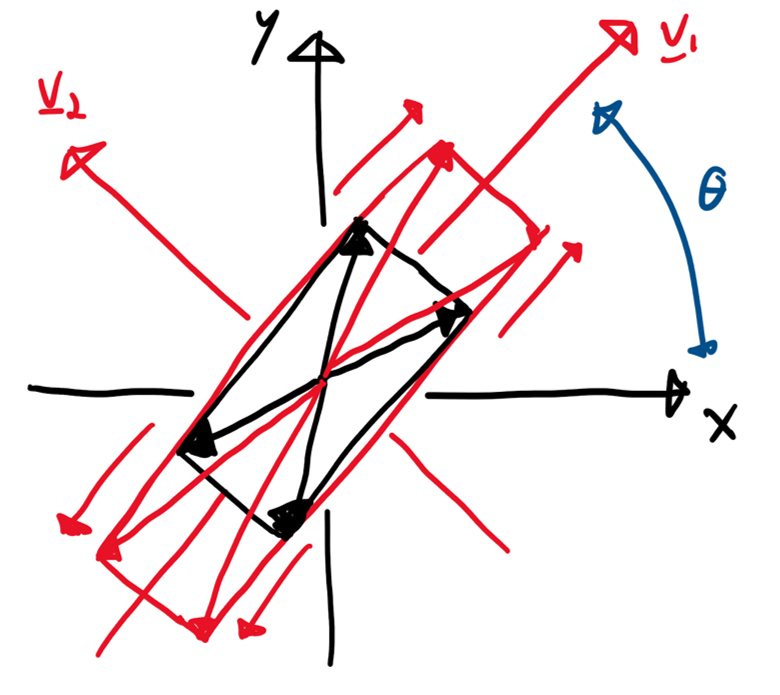
\includegraphics[width=0.55\textwidth]{linalgebra_diag_exemple.png}
	\caption{Exemple de diagonalisation pour une transformation géométrique}
	\label{fig:linalgebra_diag_exemple}
\end{figure}
%%%%%%%%%%%%%%%%%%%%%%%%%%%%%%%%%%%%%%%%%%%%%%%%%%%%%%%%%%%%%

%%%%%%%%%%%%%%%%%%%%%%%%%%%
\begin{align}
A =
\left[ \begin{array}{c c}  
c\theta^2+1     & c\theta s\theta \\
c\theta s\theta & s\theta^2+1
\end{array} \right]
=
\underbrace{
\left[ \begin{array}{c c}  
c\theta & - s\theta \\ 
s\theta &   c\theta 
\end{array} \right]
}_{V}
\;
\underbrace{
\left[ \begin{array}{c c}  
2 & 0 \\
0 & 1 
\end{array} \right]
}_{\Lambda}
\;
\underbrace{
\left[ \begin{array}{c c}  
c\theta &   s\theta \\ 
- s\theta &   c\theta 
\end{array} \right]
}_{V^{-1}}
\end{align}
%%%%%%%%%%%%%%%%%%%%%%%%%%%









%%%%%%%%%%%%%%%%%%%%%%%%%%%%%%%%%%%%%%%%%%%%%%%%%%%%%%%%%%%%
\section{Puissance d'une matrice}
%%%%%%%%%%%%%%%%%%%%%%%%%%%%%%%%%%%%%%%%%%%%%%%%%%%%%%%%%%%%

La puissance $p$ d'une matrice est définie comme la multiplication répété de $p$ copie de cette matrice. Si la matrice est diagonalisable, la puissance de la matrice $A$ est égale à
%%%%%%%%%%%%%%%%%%%%%%%%%%%
\begin{align}
A^p = V \Lambda^p V^{-1}
\label{eq:matrixpower}
\end{align}
%%%%%%%%%%%%%%%%%%%%%%%%%%%
avec:
%%%%%%%%%%%%%%%%%%%%%%%%%%%
\begin{align}
\Lambda^p = 
\left[ \begin{array}{c c c c}  
\lambda_1^p t &  0          & 0 & 0 \\
0         &  \lambda_2^p  & 0      & 0 \\
0         &  0          &\ddots  & 0 \\
0         &  0          & 0  & \lambda_n^p
\end{array} \right]
\end{align}
%%%%%%%%%%%%%%%%%%%%%%%%%%

Cette propriété découle de la diagonalisation:
%%%%%%%%%%%%%%%%%%%%%%%%%%%
\begin{align}
A^p = A \; A \; \hdots \; A = V \Lambda V^{-1} \; V \Lambda V^{-1} \;  \hdots \; V \Lambda V^{-1} = V \Lambda \Lambda   \hdots \Lambda V^{-1} = V \Lambda^p V^{-1}
\end{align}
%%%%%%%%%%%%%%%%%%%%%%%%%%%

%%%%%%%%%%%%%%%%%%%%%%%%%%%%%%%%%%%%%%%%%%%%%%%%%%%%%%
\subsection{Exemple de calcul de l'évolution d'un système discret}
%%%%%%%%%%%%%%%%%%%%%%%%%%%%%%%%%%%%%%%%%%%%%%%%%%%%%%

La suite de Fibonacci est définie par une séquence de chiffre pour lequel le prochain est la somme des deux précédents:
%%%%%%%%%%%%%%%%%%%%%%%%%%%
\begin{align}
0 \; 1\;1\;2\;3\;5\;8\;13\;21\;34\;55
\end{align}
%%%%%%%%%%%%%%%%%%%%%%%%%%%
Le chiffre suivant est calculé en fonction des deux précédents:
%%%%%%%%%%%%%%%%%%%%%%%%%%%
\begin{align}
f_{k+1} = f_{k} + f_{k-1}
\end{align}
%%%%%%%%%%%%%%%%%%%%%%%%%%%
il faut donc un vecteur d'état $\col{x}$ de deux variable ($f_{k}$ et $f_{k-1}$ ) pour prédire le prochain chiffre. L'évolution du vecteur d'état peut être décrite par l'équation matricielle suivante:
%%%%%%%%%%%%%%%%%%%%%%%%%%%
\begin{align}
\underbrace{
\left[ \begin{array}{c}  
f_{k+1} \\ f_{k}
\end{array} \right]
}_{\col{x}_{k+1}}
=
\underbrace{
\left[ \begin{array}{c c}  
1 & 1 \\ 1 & 0 
\end{array} \right]
}_{A}
\underbrace{
\left[ \begin{array}{c}  
f_{k} \\ f_{k-1}
\end{array} \right]
}_{\col{x}_{k}}
\end{align}
%%%%%%%%%%%%%%%%%%%%%%%%%%%

Il est possible de calculer la valeur future d'une évolution discrète comme celle-ci sans calculer toute la séquence grâce la propriété \eqref{eq:matrixpower}:
%%%%%%%%%%%%%%%%%%%%%%%%%%%
\begin{align}
\col{x}_{k+1} &= A \col{x}_{k} \\
\col{x}_{k+2} &= A \col{x}_{k+1} = A A \col{x}_{k} \\
\col{x}_{k+3} &= A \col{x}_{k+2} = A A A \col{x}_{k} \\
\col{x}_{k+p} &= A^p \col{x}_{k} = V \Lambda^p V^{-1} \col{x}_{k}
\label{eq:discretevolutionpower}
\end{align}
%%%%%%%%%%%%%%%%%%%%%%%%%%%
Pour la suite de Fibonacci, la matrice $A$ qui décrit l'évolution peut être diagonalisée. Premièrement on détermine les valeurs propres:
%%%%%%%%%%%%%%%%%%%%%%%%%%%
\begin{align}
0
=
det(A - \lambda I) 
=
det\left(
\left[ \begin{array}{c c}  
1-\lambda & 1 \\ 1 & -\lambda  
\end{array} \right]
\right)
= 
\lambda^2 - \lambda -1 
\end{align}
%%%%%%%%%%%%%%%%%%%%%%%%%%%
Il y a donc deux solutions:
%%%%%%%%%%%%%%%%%%%%%%%%%%%
\begin{align}
\lambda_1 = \frac{1 + \sqrt{5}}{2} = 1.61803399 \quad\quad \lambda_2 = \frac{1 - \sqrt{5}}{2} = -0.61803399
\end{align}
%%%%%%%%%%%%%%%%%%%%%%%%%%%
ou la première valeur propre est égale au très fameux nombre d'or. Il est possible de déterminer les vecteurs propres associé en substituant dans l'équation $A \col{v} = \lambda \col{v}$, on trouve alors:
%%%%%%%%%%%%%%%%%%%%%%%%%%%
\begin{align}
\col{v}_1 = 
\left[ \begin{array}{c}  
\lambda_1 \\ 1
\end{array} \right]
\quad\quad 
\col{v}_2 = 
\left[ \begin{array}{c}  
\lambda_2 \\ 1 
\end{array} \right]
\end{align}
%%%%%%%%%%%%%%%%%%%%%%%%%%%
Il est donc maintenant possible de calculer n'importe quel position future dans la séquence directement grâce à l'équation \eqref{eq:discretevolutionpower}. Si on cherche la position $p=1E9$ à partir du début de la suite de Fibonacci:
%%%%%%%%%%%%%%%%%%%%%%%%%%%
\begin{align}
\col{x}_{p} &= V \Lambda^p V^{-1} \col{x}_{0} \\
\left[ \begin{array}{c}  
f_p \\ f_{p-1}
\end{array} \right]
&= 
\left[ \begin{array}{c c }  
\lambda_1 & \lambda_2 \\
1         & 1 \\
\end{array} \right]
\left[ \begin{array}{c c }  
\lambda_1^p & 0 \\
0         & \lambda_2^p \\
\end{array} \right]
\left[ \begin{array}{c c }  
\lambda_1 & \lambda_2 \\
1         & 1 \\
\end{array} \right]^{-1} 
\left[ \begin{array}{c}  
1 \\ 0
\end{array} \right]
\end{align}
%%%%%%%%%%%%%%%%%%%%%%%%%%%
lorsque $p$ est très grand il est possible de simplifier le calcul en négligeant la contribution $\lambda_2^p \approx 0$ puisque lorsque que la valeur absolue de la base est inférieur à l'unité, la puissance tend vers zéro lorsque $p$ tend vers l'infini. Il est donc possible de simplifier:
%%%%%%%%%%%%%%%%%%%%%%%%%%%
\begin{align}
\left[ \begin{array}{c}  
f_p \\ f_{p-1}
\end{array} \right]
&= 
\left[ \begin{array}{c c }  
\lambda_1 & \lambda_2 \\
1         & 1 \\
\end{array} \right]
\left[ \begin{array}{c c }  
\lambda_1^p & 0 \\
0         & 0 \\
\end{array} \right]
\frac{1}{\lambda_1 - \lambda_2}
\left[ \begin{array}{c c }  
1 & -\lambda_2 \\
-1         & \lambda_1 \\
\end{array} \right] 
\left[ \begin{array}{c}  
1 \\ 0
\end{array} \right]
\\
\left[ \begin{array}{c}  
f_p \\ f_{p-1}
\end{array} \right]
&= 
\left[ \begin{array}{c c}  
\lambda_1^{p+1} & 0 \\
\lambda_1^{p}  & 0\\
\end{array} \right]
\frac{1}{\lambda_1 - \lambda_2}
\left[ \begin{array}{c }  
1  \\
-1   \\
\end{array} \right] 
\\
\left[ \begin{array}{c}  
f_p \\ f_{p-1}
\end{array} \right]
&= 
\frac{1}{\lambda_1 - \lambda_2}
\left[ \begin{array}{c}  
\lambda_1^{p+1}\\
\lambda_1^{p} \\
\end{array} \right] 
\end{align}
%%%%%%%%%%%%%%%%%%%%%%%%%%%
Il est donc possible de calculer directement la valeur dans la suite pour une positon $p$ lorsque $p$ est très grand:
%%%%%%%%%%%%%%%%%%%%%%%%%%%
\begin{align}
f_p = \frac{\lambda_1^{p+1}}{\lambda_1 - \lambda_2} = \frac{1.618^{(p+1)}}{\sqrt{5}}
\end{align}
%%%%%%%%%%%%%%%%%%%%%%%%%%%

%%%%%%%%%%%%%%%%%%%%%%%%%%%%%%%%%%%%%%%%%%%%%%%%%%%%%%%%%%%%
\section{Exponentiel de matrice}
%%%%%%%%%%%%%%%%%%%%%%%%%%%%%%%%%%%%%%%%%%%%%%%%%%%%%%%%%%%%

%%%%%%%%%%%%%%%%%%%%%%%%%%%
\begin{align}
e^{At} = V e^{\Lambda t} V^{-1}
\end{align}
%%%%%%%%%%%%%%%%%%%%%%%%%%%

%%%%%%%%%%%%%%%%%%%%%%%%%%%
\begin{align}
e^{\Lambda t} = 
\left[ \begin{array}{c c c c}  
e^{\lambda_1 t} &  0          & 0 & 0 \\
0         &  e^{\lambda_2 t}  & 0      & 0 \\
0         &  0          &\ddots  & 0 \\
0         &  0          & 0  & e^{\lambda_n t}
\end{array} \right]
\end{align}
%%%%%%%%%%%%%%%%%%%%%%%%%%

%%%%%%%%%%%%%%%%%%%%%%%%%%%%%%%%%%%%%%%%%%%%%%%%%%%%%%%%%%%%
\newpage
\section{Exercices}
%%%%%%%%%%%%%%%%%%%%%%%%%%%%%%%%%%%%%%%%%%%%%%%%%%%%%%%%%%%%

\subsection{Moindres carrés pour estimer un ratio de transmission}

La figure \ref{fig:exer_ls_gearbox} illustre un boiter de transmission et cinq paires de mesures angulaires à l'entrée et à la sortie. 
%%%%%%%%%%%%%%%%%%%%%
\begin{figure}[H]
	\centering
		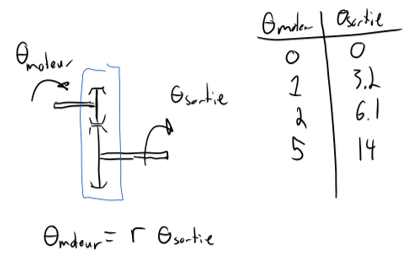
\includegraphics[width=0.50\textwidth]{exer_ls_gearbox.png}
	\caption{Moindres carrés pour estimer un ratio de transmission}
	\label{fig:exer_ls_gearbox}
\end{figure}
%%%%%%%%%%%%%%%%%%%%%%

\paragraph{A)}
Construisez le un système d'équation linéaire qui relie ces mesures expérimentales.

\paragraph{B)}
Écrivez l'équation matricielle à résoudre pour estimer le ratio de transmission.

\paragraph{C)}
Effectuer le calcul numérique pour estimer le ratio de transmission.
